\documentclass[tikz,border=6mm]{standalone}
\usepackage{amsmath,amssymb}
\usepackage{fontspec}

\usetikzlibrary{positioning,arrows.meta,shapes.geometric,fit,backgrounds,calc}

\definecolor{navyblue}{gray}{0}
\definecolor{tealblue}{gray}{0}
\definecolor{purplecat}{gray}{0}
\definecolor{ambergold}{gray}{0}
\definecolor{forestgreen}{gray}{0}
\definecolor{crimsonred}{gray}{0}
\definecolor{slategrey}{gray}{0}

\colorlet{datagreen}{tealblue}
\colorlet{modelblue}{navyblue}
\colorlet{trainpurple}{purplecat}
\colorlet{serveorange}{ambergold}
\colorlet{logslate}{slategrey}

\begin{document}
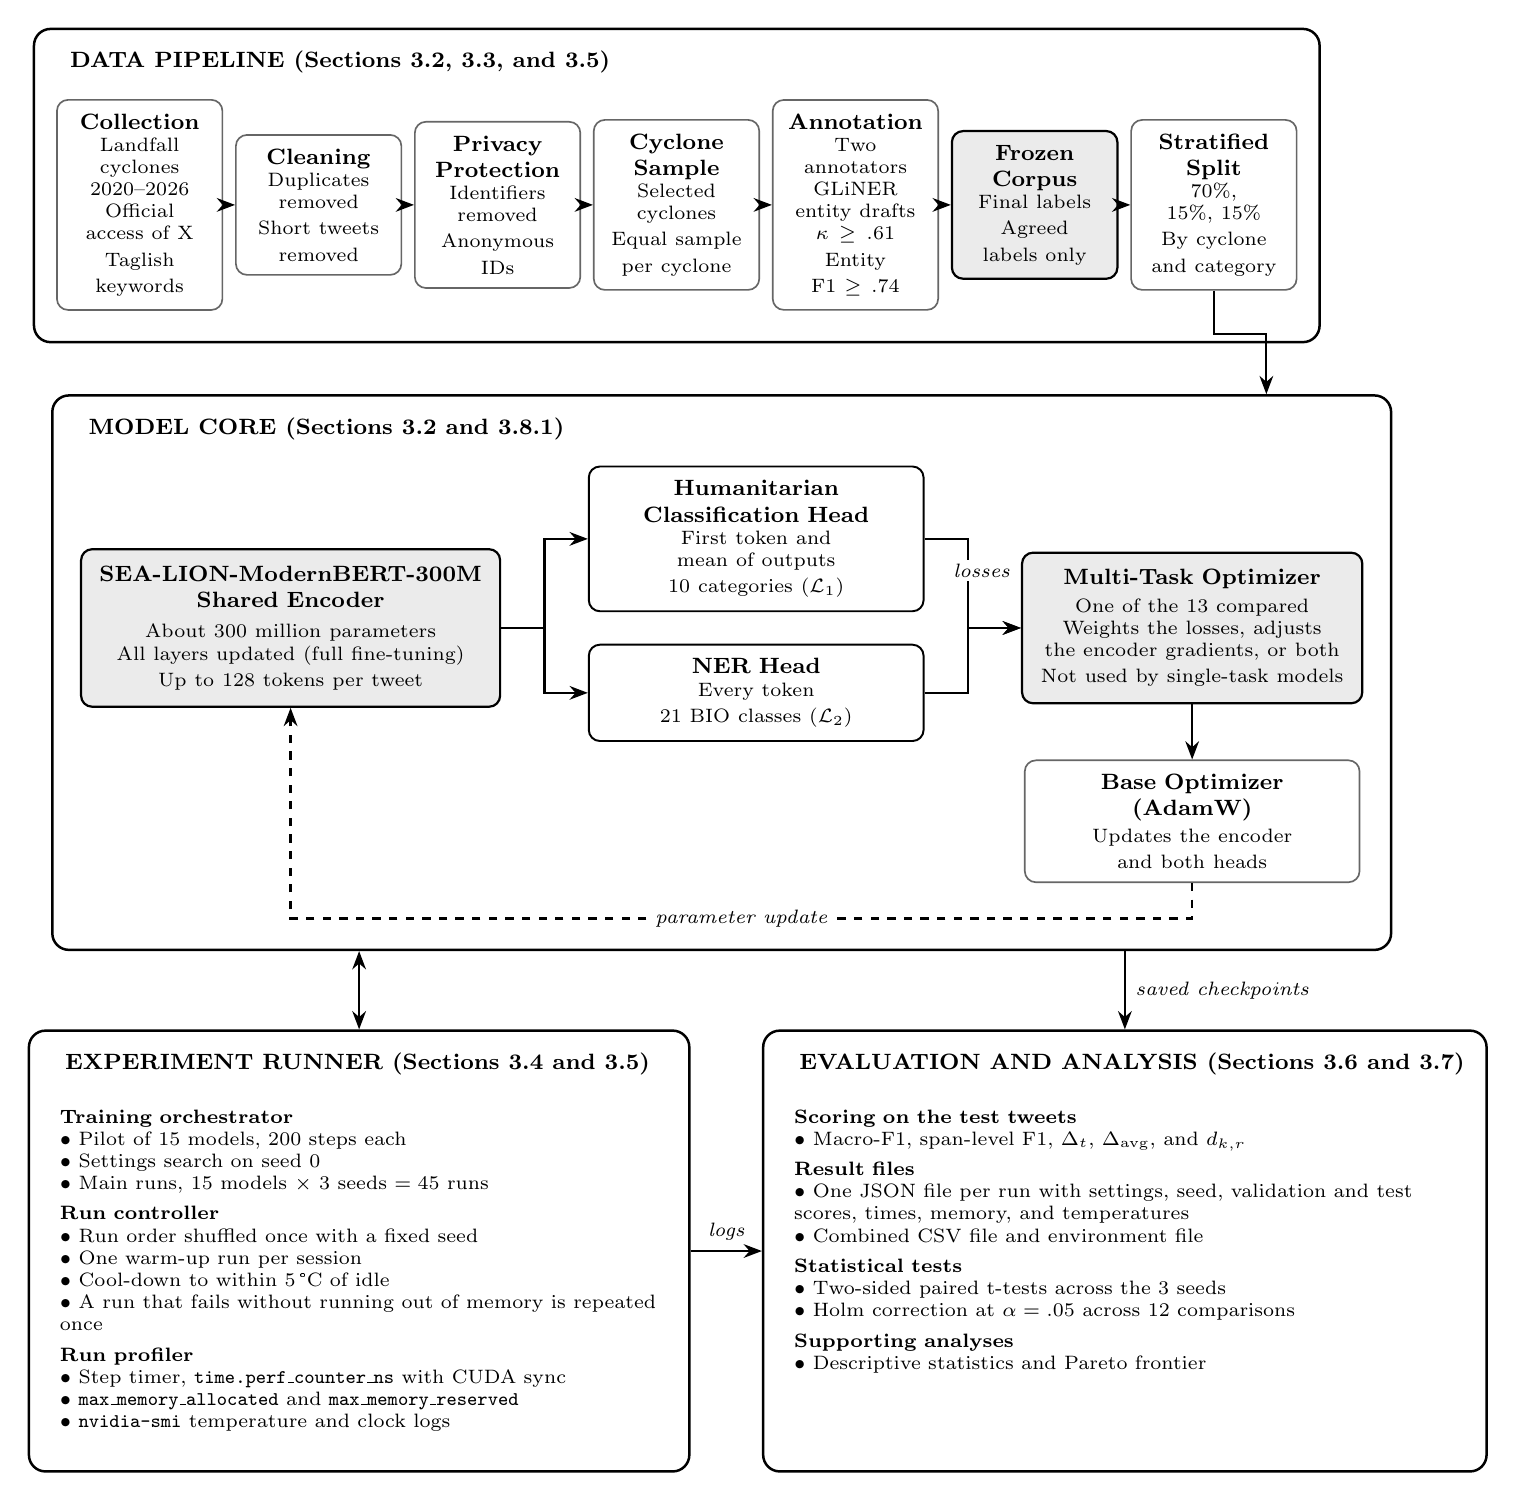
\begin{tikzpicture}[
    font=\small,
    >=Stealth,
    every node/.append style={execute at begin node={\hyphenpenalty=10000\exhyphenpenalty=10000}},
    subbox/.style={
        draw=black,
        fill=white,
        rounded corners=6pt,
        line width=0.9pt
    },
    titlelabel/.style={
        font=\bfseries\footnotesize,
        text=black,
        anchor=north west
    },
    proc/.style={
        draw=black!60,
        fill=white,
        rounded corners=4pt,
        align=center,
        inner sep=5pt,
        font=\footnotesize,
        line width=0.6pt
    },
    store/.style={
        draw=black,
        fill=black!8,
        rounded corners=4pt,
        align=center,
        inner sep=5pt,
        font=\footnotesize,
        line width=0.8pt
    },
    corenode/.style={
        draw=black,
        fill=black!8,
        rounded corners=4pt,
        align=center,
        inner sep=6pt,
        font=\footnotesize,
        line width=0.8pt
    },
    headnode/.style={
        draw=modelblue!80!black,
        fill=white,
        rounded corners=4pt,
        align=center,
        inner sep=5pt,
        font=\footnotesize,
        line width=0.7pt
    },
    itemnode/.style={
        align=left,
        inner sep=3pt,
        font=\scriptsize
    },
    arrow/.style={
        ->,
        thick,
        draw=black
    },
    biarrow/.style={
        <->,
        thick,
        draw=black
    },
    edgelabel/.style={
        font=\scriptsize\itshape,
        fill=white,
        inner sep=1.5pt
    }
]
    \node[proc, text width=1.75cm] (dp1) {
        \textbf{Collection}\\
        \scriptsize Landfall cyclones\\
        \scriptsize 2020--2026\\
        \scriptsize Official access of X\\
        \scriptsize Taglish keywords
    };

    \node[proc, right=0.15cm of dp1, text width=1.75cm] (dp2) {
        \textbf{Cleaning}\\
        \scriptsize Duplicates removed\\
        \scriptsize Short tweets removed
    };

    \node[proc, right=0.15cm of dp2, text width=1.75cm] (dp4) {
        \textbf{Privacy Protection}\\
        \scriptsize Identifiers removed\\
        \scriptsize Anonymous IDs
    };

    \node[proc, right=0.15cm of dp4, text width=1.75cm] (dp5) {
        \textbf{Cyclone Sample}\\
        \scriptsize Selected cyclones\\
        \scriptsize Equal sample per cyclone
    };

    \node[proc, right=0.15cm of dp5, text width=1.75cm] (dp6) {
        \textbf{Annotation}\\
        \scriptsize Two annotators\\
        \scriptsize GLiNER entity drafts\\
        \scriptsize $\kappa \geq .61$\\
        \scriptsize Entity F1 $\geq .74$
    };

    \node[store, right=0.15cm of dp6, text width=1.75cm] (dp7) {
        \textbf{Frozen Corpus}\\
        \scriptsize Final labels\\
        \scriptsize Agreed labels only
    };

    \node[proc, right=0.15cm of dp7, text width=1.75cm] (dp8) {
        \textbf{Stratified Split}\\
        \scriptsize 70\%, 15\%, 15\%\\
        \scriptsize By cyclone and category
    };

    \draw[arrow] (dp1) -- (dp2);
    \draw[arrow] (dp2) -- (dp4);
    \draw[arrow] (dp4) -- (dp5);
    \draw[arrow] (dp5) -- (dp6);
    \draw[arrow] (dp6) -- (dp7);
    \draw[arrow] (dp7) -- (dp8);

    \begin{scope}[on background layer]
        \node[subbox=datagreen,
              fit={(dp1) (dp8) ([yshift=22pt]dp1.north) ([yshift=-8pt]dp1.south)},
              inner xsep=8pt] (databox) {};
    \end{scope}
    \node[titlelabel=datagreen] at ([xshift=10pt, yshift=-5pt]databox.north west)
        {DATA PIPELINE (Sections 3.2, 3.3, and 3.5)};

    \node[corenode, text width=4.9cm, anchor=north west] (encoder)
        at ($(databox.south west)+(0.6,-2.6)$) {
        \textbf{SEA-LION-ModernBERT-300M Shared Encoder}\\[3pt]
        \scriptsize About 300 million parameters\\
        \scriptsize All layers updated (full fine-tuning)\\
        \scriptsize Up to 128 tokens per tweet
    };

    \node[headnode, text width=3.9cm, anchor=south west] (head_class)
        at ($(encoder.east)+(1.1,0.2)$) {
        \textbf{Humanitarian Classification Head}\\
        \scriptsize First token and mean of outputs\\
        \scriptsize 10 categories ($\mathcal{L}_1$)
    };

    \node[headnode, text width=3.9cm, anchor=north west] (head_ner)
        at ($(encoder.east)+(1.1,-0.2)$) {
        \textbf{NER Head}\\
        \scriptsize Every token\\
        \scriptsize 21 BIO classes ($\mathcal{L}_2$)
    };

    \node[corenode, text width=3.9cm, anchor=west] (mto)
        at ($(encoder.east)+(6.6,0)$) {
        \textbf{Multi-Task Optimizer}\\[2pt]
        \scriptsize One of the 13 compared\\
        \scriptsize Weights the losses, adjusts the encoder gradients, or both\\
        \scriptsize Not used by single-task models
    };

    \node[proc, text width=3.9cm, below=0.7cm of mto] (adamw) {
        \textbf{Base Optimizer (AdamW)}\\
        \scriptsize Updates the encoder and both heads
    };

    \draw[arrow] (encoder.east) -- ++(0.55,0) |- (head_class.west);
    \draw[arrow] (encoder.east) -- ++(0.55,0) |- (head_ner.west);

    \draw[arrow] (head_class.east) -- ++(0.55,0) |- (mto.west);
    \draw[arrow] (head_ner.east) -- ++(0.55,0) |- (mto.west);
    \node[edgelabel, above=1pt] at ($(mto.west)+(-0.5,0.55)$) {losses};

    \draw[arrow] (mto.south) -- (adamw.north);
    \coordinate (updturn) at ($(adamw.south)+(0,-0.45)$);
    \draw[arrow, dashed] (adamw.south) -- (updturn) -| (encoder.south)
        node[pos=0.25, edgelabel] {parameter update};

    \begin{scope}[on background layer]
        \node[subbox=modelblue,
              fit={(encoder) (head_class) (head_ner) (mto) (adamw) (updturn)
                   ([yshift=22pt]head_class.north) ([yshift=-8pt]updturn)},
              inner xsep=10pt] (modelbox) {};
    \end{scope}
    \node[titlelabel=modelblue] at ([xshift=10pt, yshift=-5pt]modelbox.north west)
        {MODEL CORE (Sections 3.2 and 3.8.1)};

    \draw[arrow] (dp8.south) -- ++(0,-0.55) -| ([xshift=-1.6cm]modelbox.north east);

    \node[itemnode, anchor=north west, text width=7.6cm] (runtext)
        at ($(modelbox.south west)+(0,-1.9)$) {
        \textbf{Training orchestrator}\\
        $\bullet$ Pilot of 15 models, 200 steps each\\
        $\bullet$ Settings search on seed 0\\
        $\bullet$ Main runs, 15 models $\times$ 3 seeds $= 45$ runs\\[3pt]
        \textbf{Run controller}\\
        $\bullet$ Run order shuffled once with a fixed seed\\
        $\bullet$ One warm-up run per session\\
        $\bullet$ Cool-down to within 5\,\textdegree C of idle\\
        $\bullet$ A run that fails without running out of memory is repeated once\\[3pt]
        \textbf{Run profiler}\\
        $\bullet$ Step timer, \texttt{time.perf\_counter\_ns} with CUDA sync\\
        $\bullet$ \texttt{max\_memory\_allocated} and \texttt{max\_memory\_reserved}\\
        $\bullet$ \texttt{nvidia-smi} temperature and clock logs
    };

    \begin{scope}[on background layer]
        \node[subbox=trainpurple,
              fit={(runtext) ([yshift=22pt]runtext.north) ([yshift=-8pt]runtext.south)},
              inner xsep=8pt] (runbox) {};
    \end{scope}
    \node[titlelabel=trainpurple] at ([xshift=10pt, yshift=-5pt]runbox.north west)
        {EXPERIMENT RUNNER (Sections 3.4 and 3.5)};

    \node[itemnode, anchor=north west, text width=8.4cm] (evaltext)
        at ($(runtext.north east)+(1.5,0)$) {
        \textbf{Scoring on the test tweets}\\
        $\bullet$ Macro-F1, span-level F1, $\Delta_t$, $\Delta_{\text{avg}}$, and $d_{k,r}$\\[3pt]
        \textbf{Result files}\\
        $\bullet$ One JSON file per run with settings, seed, validation and test scores, times, memory, and temperatures\\
        $\bullet$ Combined CSV file and environment file\\[3pt]
        \textbf{Statistical tests}\\
        $\bullet$ Two-sided paired t-tests across the 3 seeds\\
        $\bullet$ Holm correction at $\alpha = .05$ across 12 comparisons\\[3pt]
        \textbf{Supporting analyses}\\
        $\bullet$ Descriptive statistics and Pareto frontier
    };

    \begin{scope}[on background layer]
        \node[subbox=serveorange,
              fit={(evaltext) (runtext.south -| evaltext.west) ([yshift=22pt]evaltext.north) ([yshift=-8pt]runtext.south -| evaltext.west)},
              inner xsep=8pt] (evalbox) {};
    \end{scope}
    \node[titlelabel=serveorange] at ([xshift=10pt, yshift=-5pt]evalbox.north west)
        {EVALUATION AND ANALYSIS (Sections 3.6 and 3.7)};

    \draw[biarrow] (modelbox.south -| runbox.center) -- (runbox.north);
    \draw[arrow] (modelbox.south -| evalbox.center) -- (evalbox.north)
        node[midway, right=2pt, edgelabel] {saved checkpoints};
    \draw[arrow] (runbox.east) -- (runbox.east -| evalbox.west)
        node[midway, above=2pt, edgelabel] {logs};

\end{tikzpicture}
\end{document}
